\renewcommand{\appendixsname}{Appendix}
\chapter{Generated ResourceManager Graphs}
\label{chap:ApendA}

Following there are a brief explanation and the figures that were generated through the second method employed on the section \ref{sec:grafo}.

The pertinence of these figures is validated by the fact that they describe all possible ways a given interface can take. The perfect case flow would be started with the submission of a job to the RM. There are some pre requisites that need to be fulfilled for the start of the job. From this point on, these figures are relevant.

Firstly an AppAttempt is created. The AppAttempt is literally a started application, through which the RM will try to allocate necessary resources (Node and Containers). If the resources are successfully allocated, the real App will be created. Then an ApplicationMaster will be launched in order to manage each Application allocated RMContainers and to which RMNode they belong.

\begin{figure}[hbtn]
   \centering
   \renewcommand{\figurename}{Figure}
   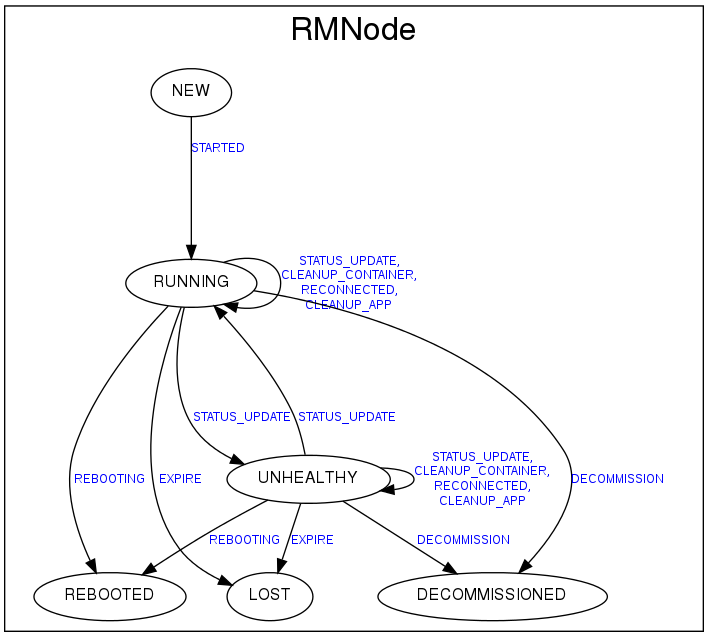
\includegraphics[width=12cm]{figuras/Figura05-RMNode.png}
   \caption{RMNode's state machine}
   \label{fig:RMNode}
\end{figure}

\begin{figure}[hbtn]
   \centering
   \renewcommand{\figurename}{Figure}
   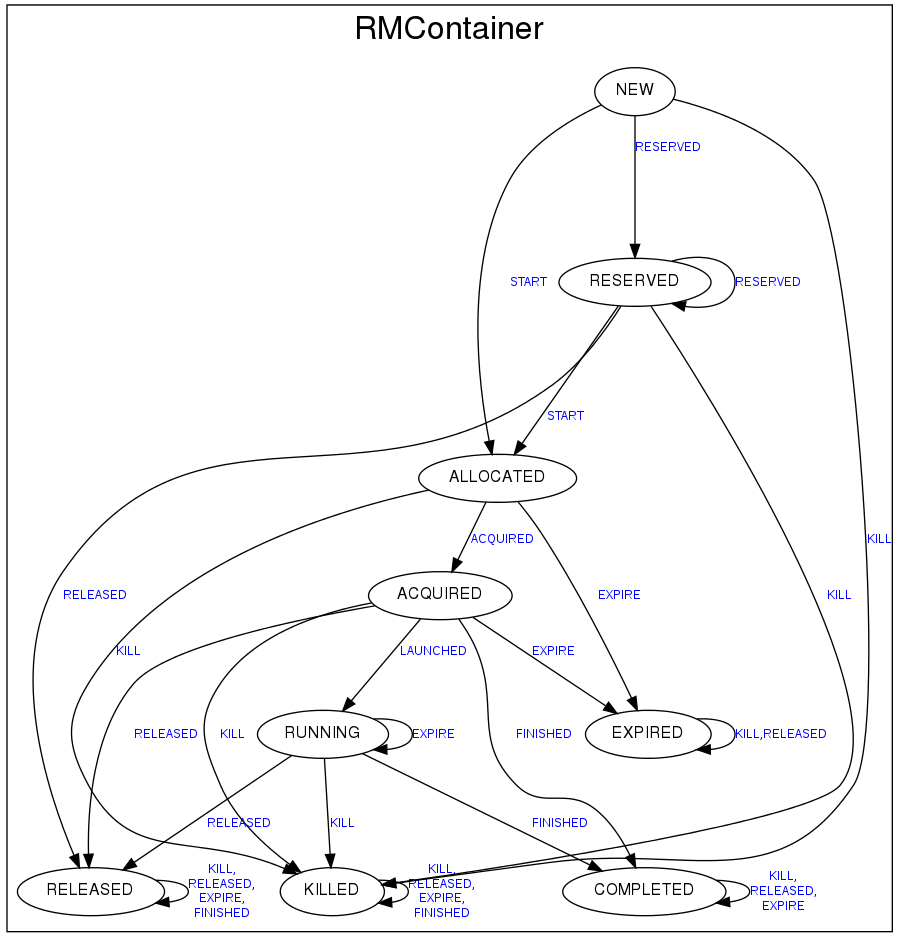
\includegraphics[width=15cm]{figuras/Figura03-RMContainer.png}
   \caption{RMContainer's state machine}
   \label{fig:RMContainer}
\end{figure}

\begin{figure}[hbtn]
   \centering
   \renewcommand{\figurename}{Figure}
   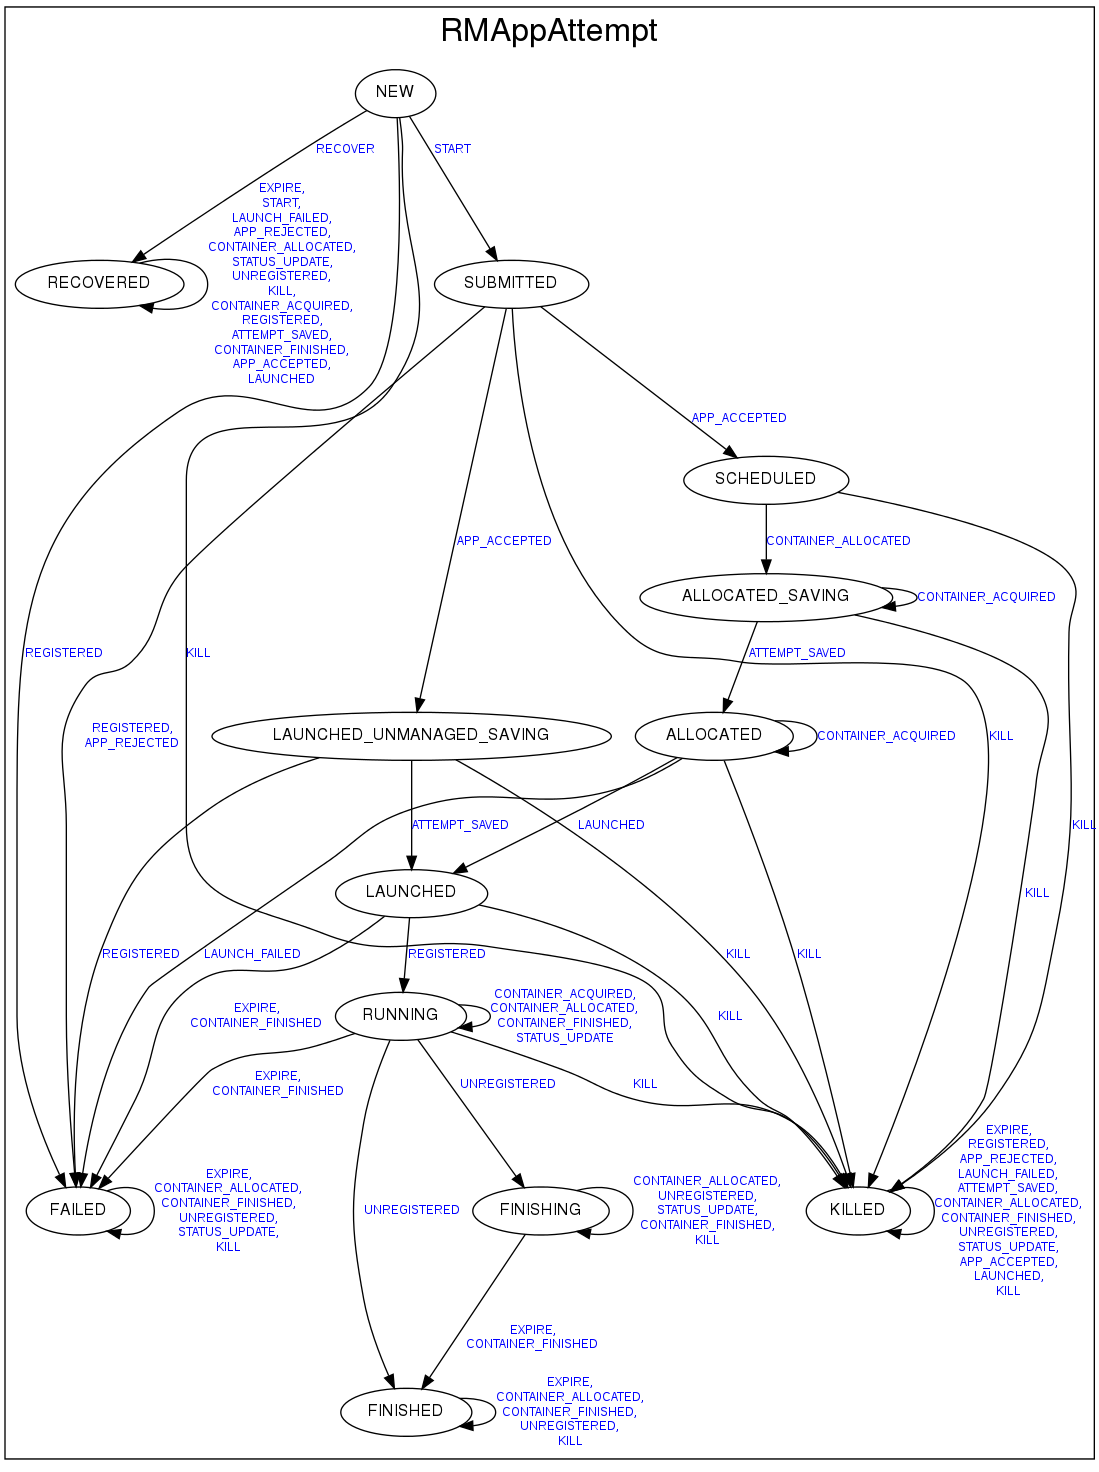
\includegraphics[width=15cm]{figuras/Figura02-RMAppAttempt.png}
   \caption{RMAppAttempt's state machine}
   \label{fig:RMAppAttempt}
\end{figure}

\begin{figure}[hbtn]
   \centering
   \renewcommand{\figurename}{Figure}
   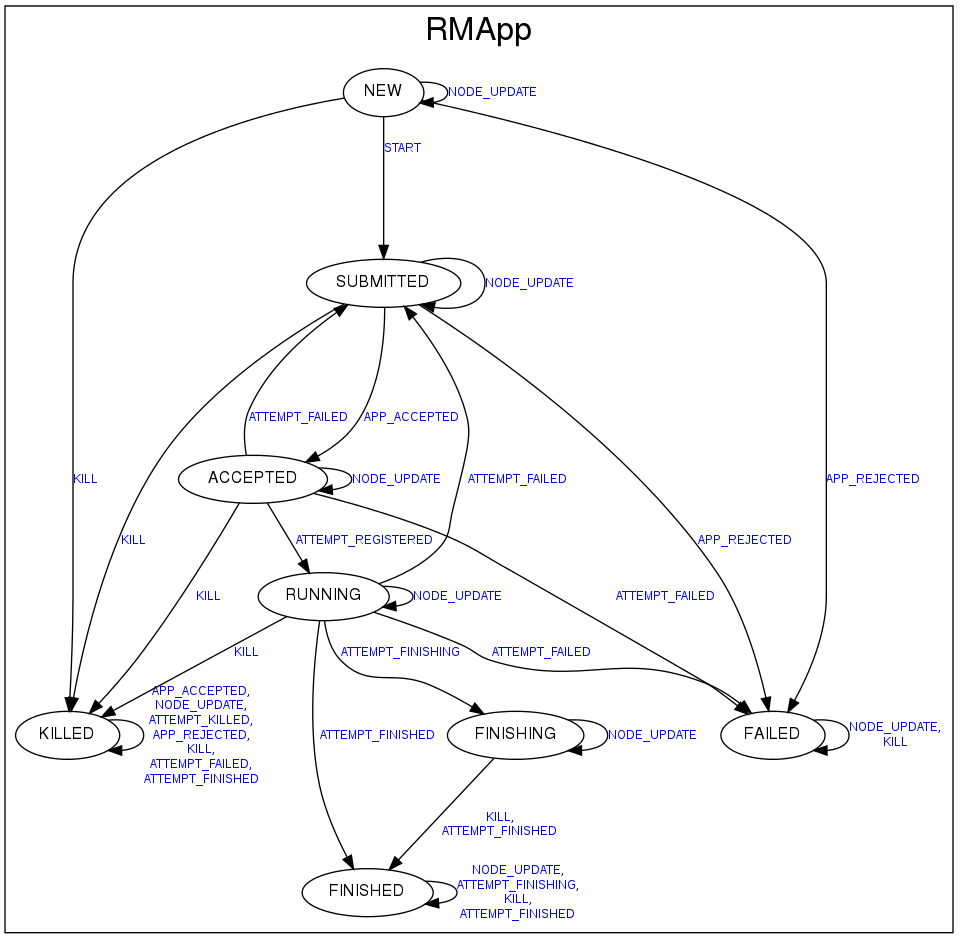
\includegraphics[width=15cm]{figuras/Figura04-RMApp.png}
   \caption{RMApp's state machine}
   \label{fig:RMApp}
\end{figure}